\documentclass[11pt]{article}
\usepackage[a4paper,margin=2.5cm]{geometry}
\usepackage[utf8]{inputenc}
\usepackage[T1]{fontenc}
\usepackage{graphicx}
\usepackage{booktabs}
\usepackage{setspace}
\onehalfspacing
\graphicspath{{figures/}}
\renewcommand{\figurename}{Supplementary Figure}
\renewcommand{\tablename}{Supplementary Table}

\title{\textbf{Supplementary Information}\\
\large Mapping intra-urban social deprivation from Sentinel imagery using only
municipal aggregate labels}
\author{}
\date{}

\begin{document}
\maketitle

\begin{figure}[h]
\centering
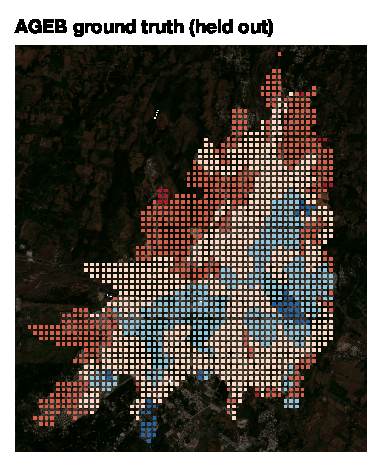
\includegraphics[width=0.62\linewidth]{fig1_truth.pdf}
\caption{Tract-level ground truth for Tapachula, on the color scale of main-text
Fig.~1c. Every token inherits the held-out GRS grade of the AGEB it falls in.}
\end{figure}

\begin{table}[h]
\centering
\caption{The supervision-efficiency curve (main-text Fig.~2a). Mean over three seeds;
validation cities were used for model selection, test cities are held out.}
\begin{tabular}{rcc}
\toprule
Bags & Validation within-$\rho$ (s.d.) & Test within-$\rho$\\
\midrule
50 & 0.150 (0.021) & 0.156\\
100 & 0.141 (0.021) & 0.158\\
200 & 0.151 (0.022) & 0.161\\
400 & 0.182 (0.020) & 0.192\\
771 & 0.227 (0.010) & 0.185 (retrained); 0.196 (saved weights)\\
\bottomrule
\end{tabular}
\end{table}

\begin{table}[h]
\centering
\caption{Agreement by tract size (main-text Limits). Within-municipality Spearman over
municipalities with at least ten tracts in the bin.}
\begin{tabular}{rrrrc}
\toprule
Tokens per tract & Tracts & Median population & Municipalities & Within-$\rho$\\
\midrule
1--3 & 567 & 211 & 15 & 0.257\\
4--9 & 849 & 1{,}948 & 16 & 0.338\\
10--19 & 999 & 2{,}644 & 20 & 0.352\\
20--49 & 464 & 3{,}231 & 14 & 0.432\\
$\geq$50 & 79 & 3{,}561 & 2 & 0.127\\
\bottomrule
\end{tabular}
\end{table}

\begin{table}[h]
\centering
\caption{Municipalities excluded from the expansion for insufficient optical depth or
persistent acquisition errors; the guard requires eight observations per pixel and
excludes shallow ground instead of compositing it.}
\begin{tabular}{ll}
\toprule
Municipality & Reason\\
\midrule
Amozoc; Comalcalco; Hidalgo del Parral; & composite below the eight-observation\\
Lagos de Moreno; Nuevo Casas Grandes & depth floor (optical arm)\\
La Independencia & inconsistent tract geometry\\
El Marqu\'es & repeated acquisition timeouts\\
\bottomrule
\end{tabular}
\end{table}

\begin{table}[h]
\centering
\caption{Free global products under the map's own protocol. Within-$\rho$ is the mean
over municipalities of the within-municipality Spearman correlation against the held-out
tract grade, on the identical universe; $\Delta$ is the paired difference with a
city-clustered bootstrap interval; AUROC is pooled detection of high and very-high grade
tracts across the split. Orientation was fixed before measurement: deprivation is the
negative of every product. The nighttime-light row rests on interior-point sampling for 63\%
of tracts, which are smaller than one of its 30 arcsec cells.}
\begin{tabular}{lccccc}
\toprule
Product & Split & Map & Product & $\Delta$ [95\% CI] & AUROC map / product\\
\midrule
GHSL built-up surface & val & 0.354 & 0.202 & $+0.152$ [$-0.103$, $+0.303$] & 0.828 / 0.866\\
 & test & 0.232 & 0.174 & $+0.059$ [$-0.098$, $+0.160$] & 0.829 / 0.908\\
GHSL building height & val & 0.354 & 0.226 & $+0.128$ [$-0.096$, $+0.291$] & 0.828 / 0.859\\
 & test & 0.232 & 0.119 & $+0.113$ [$-0.062$, $+0.233$] & 0.829 / 0.886\\
GHSL population & val & 0.354 & 0.065 & $+0.289$ [$-0.001$, $+0.497$] & 0.828 / 0.872\\
 & test & 0.232 & 0.045 & $+0.188$ [$+0.051$, $+0.289$] & 0.829 / 0.855\\
Nighttime lights & val & 0.364 & 0.327 & $+0.037$ [$-0.109$, $+0.149$] & 0.828 / 0.840\\
 & test & 0.210 & 0.249 & $-0.039$ [$-0.245$, $+0.104$] & 0.829 / 0.831\\
\bottomrule
\end{tabular}
\end{table}

\begin{table}[h]
\centering
\caption{Conformal grade intervals at 90\% nominal coverage, calibrated on the validation
cities and evaluated on the test cities. The marginal rule assumes all tracts
exchangeable; the clustered rule takes each calibration city's quantile and then the 90th
percentile across cities.}
\begin{tabular}{lccccc}
\toprule
Rule & Half-width (grades) & Coverage & Worst city & Worst city coverage & Cities below\\
\midrule
Marginal & 1.29 & 0.869 & La Paz & 0.768 & 10 of 14\\
Clustered by city & 1.68 & 0.953 & Madera & 0.870 & 1 of 14\\
\bottomrule
\end{tabular}
\end{table}

\begin{table}[h]
\centering
\caption{The fourteen test cities ranked by the within-municipality correlation their map
achieves, worst first. Tract-mean scores. Spread is the median across tracts of the
standard deviation over three seeds, which does not separate the failures from the
successes.}
\begin{tabular}{lrrrr}
\toprule
City & Municipalities & Tracts & Within-$\rho$ & Median seed spread\\
\midrule
Guerrero & 1 & 21 & $-0.510$ & 0.101\\
Ciudad del Carmen & 1 & 54 & $-0.267$ & 0.069\\
Esc\'arcega & 1 & 24 & $-0.001$ & 0.093\\
Madera & 1 & 46 & $0.052$ & 0.133\\
Quer\'etaro & 3 & 514 & $0.091$ & 0.109\\
Zapopan & 2 & 335 & $0.105$ & 0.104\\
Garc\'ia & 3 & 324 & $0.257$ & 0.088\\
Nogales & 1 & 171 & $0.261$ & 0.093\\
Victoria & 1 & 165 & $0.373$ & 0.102\\
Hidalgo & 1 & 71 & $0.425$ & 0.098\\
Irapuato & 1 & 214 & $0.465$ & 0.121\\
Ixtapaluca & 4 & 463 & $0.471$ & 0.097\\
La Paz & 1 & 276 & $0.534$ & 0.095\\
Iguala de la Independencia & 1 & 133 & $0.639$ & 0.125\\
\bottomrule
\end{tabular}
\end{table}


\begin{table}[h]
\centering
\caption{Global products offered to the model as input features, validation cities,
within-municipality Spearman, three seeds. GHSL built-up surface, building height,
population and nighttime lights as four token columns; WorldCover as its eleven class
fractions plus NDVI mean and dispersion. The oracle rows are standardised, with their
own no-extras reference; the paired difference is per municipality, seed-averaged, with a
city-clustered bootstrap. The map rows fuse the columns either into the projection
(early) or straight into the scoring layer (late).}
\begin{tabular}{llccc}
\toprule
Head & Extra inputs & Seeds & Mean & Paired difference [95\%]\\
\midrule
Oracle & none (reference) & 0.288 / 0.239 / 0.257 & 0.261 & \\
Oracle & WorldCover & 0.288 / 0.261 / 0.272 & 0.274 & $+0.014$ [$-0.004$, $+0.030$]\\
Oracle & GHSL + lights & 0.293 / 0.281 / 0.298 & 0.291 & $+0.030$ [$+0.011$, $+0.050$]\\
Oracle & both & 0.291 / 0.278 / 0.300 & 0.289 & $+0.030$ [$+0.012$, $+0.046$]\\
\midrule
Map & none (canonical) & 0.242 / 0.224 / 0.215 & 0.227 & \\
Map, early & WorldCover & 0.207 / 0.221 / 0.209 & 0.212 & \\
Map, early & GHSL + lights & 0.226 / 0.236 / 0.214 & 0.225 & \\
Map, early & both & 0.220 / 0.227 / 0.217 & 0.221 & \\
Map, late & GHSL + lights & 0.214 / 0.217 / 0.198 & 0.210 & \\
Map, late & both & 0.241 / 0.221 / 0.216 & 0.226 & \\
\bottomrule
\end{tabular}
\end{table}

\begin{table}[h]
\centering
\caption{Transfer under each country's own municipal aggregates (main-text Fig.~4d).
Within-municipality Spearman against the fine truth, grouped five-fold by municipality,
per seed; Bogot\'a's oracle folds over 3.2 km spatial cells. Colombia: 35 bags, the
Bogot\'a block strata as truth over 12{,}738 built tokens. Brazil: 48 bags, tract median
income of the household head as truth over 110{,}728 tokens in 47 municipalities, with
the municipality-bootstrap interval of the mean. AUROC is for the most deprived quartile
of the truth, pooled. The earlier zero-shot protocol, without the built-token filter,
gave $\rho = 0.318$ and AUROC 0.716 (strata 1--2) in Bogot\'a over 14{,}132 tokens and
AUROC 0.557 for Rio's mapped informal settlements over 34{,}331 built tokens.}
\begin{tabular}{llcccc}
\toprule
Country & Method & Seeds & Mean [95\%] & Pooled $\rho$ & AUROC\\
\midrule
Colombia & Mexican, unadapted & 0.311 & 0.311 & 0.311 & 0.705\\
Colombia & local aggregates & 0.223 / 0.178 / 0.238 & 0.213 & 0.213 & 0.630\\
Colombia & Mexican, fine-tuned & 0.294 / 0.138 / 0.305 & 0.246 & 0.246 & 0.660\\
Colombia & oracle & 0.741 / 0.758 / 0.749 & 0.749 & 0.749 & 0.906\\
\midrule
Brazil & Mexican, unadapted & 0.099 & 0.099 [0.048, 0.148] & 0.283 & 0.648\\
Brazil & local aggregates & 0.115 / 0.119 / 0.130 & 0.121 [0.074, 0.171] & 0.332 & 0.636\\
Brazil & Mexican, fine-tuned & 0.074 / 0.077 / 0.084 & 0.078 [0.026, 0.129] & 0.337 & 0.633\\
Brazil & oracle & 0.239 / 0.269 / 0.234 & 0.247 [0.197, 0.297] & 0.472 & 0.704\\
\bottomrule
\end{tabular}
\end{table}

\end{document}
